\documentclass[border=5pt]{standalone}

\usepackage{amsfonts,amssymb,amsmath}
\usepackage{tikz}
\usetikzlibrary{matrix}

\newcommand{\BO}{\mathrm{BO}}
\newcommand{\BSO}{\mathrm{BSO}}
\newcommand{\BSpin}{\mathrm{BSpin}}

\newcommand{\zz}{\ensuremath\mathbb{Z}_2}
\newcommand{\Z}{\ensuremath\mathbb{Z}}

\tikzset{ 
table/.style={
  matrix of nodes,
  row sep=-\pgflinewidth,
  column sep=-\pgflinewidth,
  nodes={rectangle,text width=3em,align=center},
  text depth=1.25ex,
  text height=4ex,
  nodes in empty cells
},
column 1/.style={nodes={fill=gray!20,text depth=2.4ex,text width=8em}},
row 1/.style={nodes={rectangle, text height=3ex, text depth=1ex, align=center}},
row 2/.style={nodes={rectangle, text height=1ex, text depth=1ex, align=center}},
row 6/.style={nodes={rectangle, text height=2ex, text depth=1ex, align=center}},
row 7/.style={nodes={rectangle, text height=2ex, text depth=1ex, align=center}},
row 8/.style={nodes={rectangle, text height=2ex, text depth=1ex, align=center}}
%column 6/.style={nodes={rectangle, text width=3em,align=center}},
%column 7/.style={nodes={rectangle, text width=3em,align=center}},
%column 2/.style={nodes={rectangle, text width=3em,align=center}}
}

\begin{document}
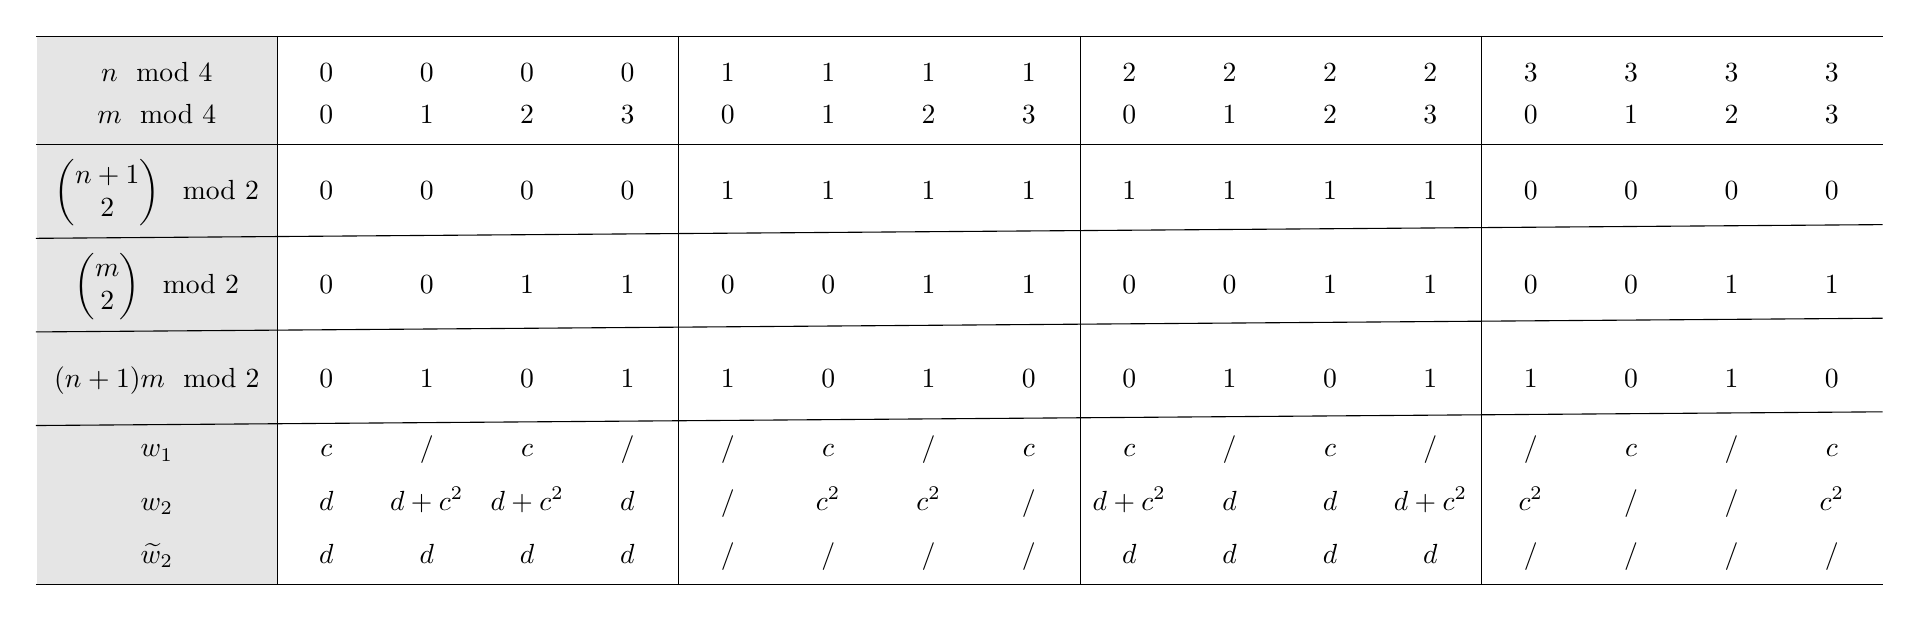
\begin{tikzpicture}
\matrix (mat) [table] {
    $n\mod 4$ & $0$ & $0$ & $0$ & $0$ & $1$ & $1$ & $1$ & $1$ & $2$ & $2$ & $2$ & $2$ & $3$ & $3$ & $3$ & $3$\\
    $m\mod 4$ & $0$ & $1$ & $2$ & $3$ & $0$ & $1$ & $2$ & $3$ & $0$ & $1$ & $2$ & $3$ & $0$ & $1$ & $2$ & $3$ \\
    $\begin{pmatrix} n + 1\\2\end{pmatrix}\mod 2$ & $0$ & $0$ & $0$ & $0$ & $1$ & $1$ & $1$ & $1$ & $1$ & $1$ & $1$ & $1$ & $0$ & $0$ & $0$ & $0$  \\
    $\begin{pmatrix}m \\2\end{pmatrix} \mod 2$ & $0$ & $0$ & $1$ & $1$ & $0$ & $0$ & $1$ & $1$ & $0$ & $0$ & $1$ & $1$ & $0$ & $0$ & $1$ & $1$ \\
    $(n+1)m\mod 2$ & $0$ & $1$ & $0$ & $1$ & $1$ & $0$ & $1$ & $0$ & $0$ & $1$ & $0$ & $1$ & $1$ & $0$ & $1$ & $0$ \\
    $w_1$ & $c$ & $/$ & $c$ & $/$ & $/$ & $c$ & $/$ & $c$ & $c$ & $/$ & $c$ & $/$ & $/$ & $c$ & $/$ & $c$ \\
    $w_2$ & $d$ & $d+c^2$ & $d+c^2$ & $d$ & $/$ & $c^2$ & $c^2$ & $/$ & $d+c^2$ & $d$ & $d$ & $d+c^2$ & $c^2$ & $/$ & $/$ & $c^2$ \\ 
    $\widetilde{w}_2$ & $d$ & $d$ & $d$ & $d$ & $/$ & $/$ & $/$ & $/$ & $d$ & $d$ & $d$ & $d$ & $/$ & $/$ & $/$ & $/$ \\
};
% the matrix rules
  \draw
    ([xshift=-.5\pgflinewidth]mat-1-1.north west) --
    ([xshift=-.5\pgflinewidth]mat-1-17.north east);
  \draw
    ([xshift=-.5\pgflinewidth]mat-8-1.south west) --
    ([xshift=-.5\pgflinewidth]mat-8-17.south east);
\foreach \x in {2,...,5}
{
  \draw
    ([xshift=-.5\pgflinewidth]mat-\x-1.south west) --
    ([xshift=-.5\pgflinewidth]mat-\x-17.south east);
  }
\draw
    ([yshift=.5\pgflinewidth]mat-1-1.north east) --
    ([yshift=.5\pgflinewidth]mat-8-1.south east);
\draw
    ([yshift=.5\pgflinewidth]mat-1-5.north east) --
    ([yshift=.5\pgflinewidth]mat-8-5.south east);
\draw
    ([yshift=.5\pgflinewidth]mat-1-9.north east) --
    ([yshift=.5\pgflinewidth]mat-8-9.south east);
\draw
    ([yshift=.5\pgflinewidth]mat-1-13.north east) --
    ([yshift=.5\pgflinewidth]mat-8-13.south east);
% the arrows
\begin{scope}[shorten >=7pt,shorten <=7pt]
\end{scope}
\end{tikzpicture}
\end{document}
